\chapter{Design}

\section{High Level Overview}
The goal of this section is to provide a high level, top down overview of the entire project. I have combined all the ideas that I have taken from the research, and compiled them down into many steps in order of priority, including algorithms and pseudocode snippets for which I may look back upon and integrate into the real process. \\
From what I have compiled, I have created an overview from the compilation of these ideas. \\

\textbf{The Project} \\
The project which I will be developing is a web based application, which contains a well presented and realistic globe representing the earth, allowing for a satellite view of the globe. The globe will appear suspended in space, upon which it can be manipulated using the mouse, where it can be rotated, moved around, and interacted with. These interactions may do many things. The dragging of the mouse, for example, will rotate the sphere, the hovering over countries will highlight them, allowing them to be clicked. Upon a mouse click, a country is selected, and useful information about the country is displayed, allowing students in analytics courses or people with interests in country data to note, all displayed in a unique manner, allowing for a unique experience. Not only may it be useful for students, or people in data science; people whom appreciate the beauty of the earth may enjoy toying around with the globe. \\
I was partially inspired by similar projects, such as Google Earth, I thought that the way the globe was represented was interesting, and thought that I may undertake in a similar project, adding my own unique twist.

\section{Description of Algorithms}
The goal of this section is to compile some algorithms written in pseudocode format, it contains a code based approach to the project problems.

\subsection{Rendering of the globe}
Before rendering the globe, we must set up the scene for which our globe can be displayed in, and we must define how the camera will see our object:
\begin{lstlisting}
GlobeScene = Scene()
Camera = PerspectiveCamera({
	field of view = 75 degrees,
	aspect ratio = WINDOW WIDTH / WINDOW HEIGHT
})

// The renderer is the HTML component where our sphere can be seen
Renderer = WebGLRenderer({
	size = WINDOW WIDTH, WINDOW HEIGHT
})
ADD Renderer TO HTML PAGE
\end{lstlisting}
The globe will be rendered in many steps, for example, the earth's sphere will be displayed, then an atmosphere will be layered, then perhaps clouds will be layered in between the atmosphere and the earth, etcetera. \\
All spheres will be initialized the same way. Taking inspiration from how \verb|THREE.js| declares 3D objects, I have a vague idea on how this will be done:
\begin{lstlisting}
Radius = 50
WorldTexture = LoadTexture("world.png")
GlobeGeometry = SphereGeometry(Radius)
GlobeMaterial = Material({
	texture = WorldTexture
	colour = NO COLOUR
})
Globe = Mesh(GlobeGeometry, GlobeMaterial)
Globe.position = 0, 0, 0
ADD Globe TO SCENE
\end{lstlisting}
The atmosphere will be another sphere, layered on top of the globe, with a slightly larger radius. The atmosphere will be rendered slightly different from the globe. Since it changes depending on where you look at it, it would be appropriate to use a shader that will colour the pixels in a way that looks like an atmosphere. \\
\textbf{Atmosphere Sphere Code}
\begin{lstlisting}
Radius = 60
AtmosphereGeometry = SphereGeometry(Radius)
AtmosphereMaterial = ShaderMaterial({
	shader = LOAD SHADERS
	colour = NO COLOUR
})
Atmosphere = Mesh(GlobeGeometry, GlobeMaterial)
Atmosphere.position = 0, 0, 0
\end{lstlisting}
\textbf{Atmosphere Shader Code} \\
This code won't be trivial. We need to think of a way of rendering an atmosphere. Firstly, what does an atmosphere look like? Let's think about this like a programmer - an atmosphere can be rendered like a transparent sphere, where a slight blue tinge can diffuse outwards towards the edges of a sphere. In short, from the eyes of a person, the sphere gets more and more transparent towards the middle of the sphere. Therefore, the sphere gets updated so that the middle looks transparent wherever you are looking from. This is where shaders come in handy, because we can work directly on the pixels procedurally, and also because we have the vertex data of the sphere, allowing us to know where all the points are on the sphere, and apply a colour to the pixels in each point depending on where the point is. \\
Let's tackle the problem of transparency. We want the blue tinge to slowly and gradually become lighter and more transparent towards the middle of the sphere, but first, we need to know how close to the 'middle' we are to the sphere. By doing some research, I have concluded that to do this, we need to know the \textbf{normal} of each point of the sphere. The \textbf{normal} of a point is the perpendicular vector from the surface of the object (in this case a sphere), here is a visual of what a normal is\footnote{https://www.scratchapixel.com/lessons/advanced-rendering/rendering-distance-fields/basic-sphere-tracer}: \\
\begin{figure}[h]
\centering
\includegraphics[width=0.2\linewidth]{images/screenshot004}
\caption{}
\label{fig:screenshot004}
\end{figure}
The 'N' represents the \textbf{normal}. Each vertex of a sphere has a normal vector, pointing \textit{away} from the sphere. This is exactly what we want, because normals that are pointing \textit{towards} us can be measured. Think of a sphere, the normals at the very edge of a sphere will point exactly left or right, where as points directly in the middle of a sphere will point towards you. For example, in the figure above, the normal is pointing slightly towards us. \\
But how do we measure how much the normal is pointing towards us? We need to use a vector operation called the \textbf{dot product}. The dot product combines two vectors into a single value, the resulting value tells you what amount of one vector \textit{goes in the direction of another vector}. For example, lets say we have a box and an inclined ramp, and we push it \textbf{up the ramp}. The box has a \textit{horizontal} component and \textit{vertical} component to the force vector. So the dot product in this case represents the total amount of force going in the \textbf{direction up the ramp}. \\
How can we integrate this knowledge into our shader code however? We need to find how much the normal to the sphere points towards us. From the camera lens, forwards is the \textbf{z axis}. Therefore, if we use the dot product against the normal and a vector where the x, y components are zero and the z component is, lets say, 1, then the resulting value will tell us how much the normal points towards us!
$$
Normal \cdot \begin{bmatrix} 0.0 \\ 0.0 \\ 1.0 \\ \end{bmatrix}
	= \textrm{Measure of how strongly the vector points towards camera}
$$
We can now use this formula and multiply the result by the colour of the atmosphere that we want, in this case, a slightly cyan colour. This is the pseudocode I came up with:
\begin{lstlisting}
Intensity = DotProduct(Normal, Vector(0, 0, 1))
Atmosphere = Vector(0, 1.2, 2.0) * Intensity
Pixel Colour = Vector(Atmosphere.XYZ, 0.5)
\end{lstlisting}

\subsection{User Input}
After the globe is rendered, we can handle our user input. We are focusing primarily on mouse input, as I feel like keyboard input is not necessary. \\
Firstly, we need to move our globe. Since the globe is a sphere, I am thinking of implementing a simple orbit control system. \\

\textbf{Orbital Controls - Rotation} \\
Orbital controls involve clamping the camera into a sphere. Thus, the camera cannot move outside the edges of the sphere. \\
Let's think of this as a two dimensional circle first:
\begin{center}
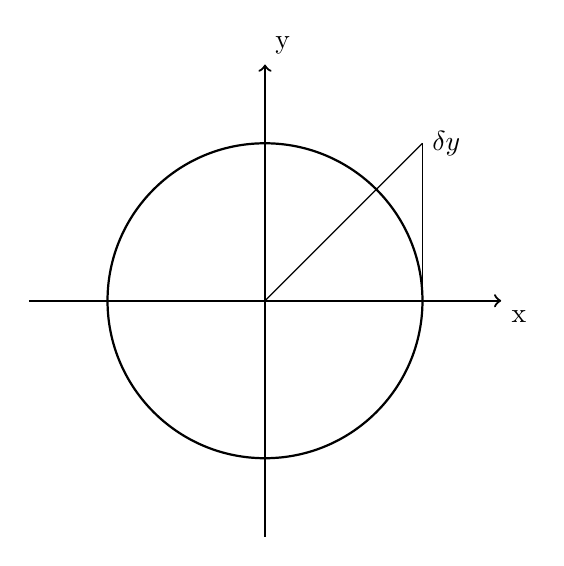
\begin{tikzpicture}
    \draw[thick, ->] (-3,0) -- (3,0) node[anchor=north west] {x};
    \draw[thick, ->] (0,-3) -- (0,3) node[anchor=south west] {y};

    \draw (0,0) -- (2,2) {};
    \draw (2,0) -- (2,2) node[right]{$\delta y$};
    \draw[thick] circle (2);
\end{tikzpicture}
\end{center}
We need to clamp the \textbf{magnitude} of the vector $\delta y$ to be equal to $R$, the radius of the circle. Therefore:
$$\frac{R}{\|\vec{\delta y}\|} \cdot \vec{\delta y} = \textrm{Clamped position}$$

\textbf{Orbital Controls - Zoom} \\
Zooming is simpler, all we need to do is add a fixed constant to our radius of the sphere, and update the camera on the scroll wheel.
$$R = R + \delta R$$

\textbf{Country detection} \\
There are two ways I can go about selecting a country on click:
\begin{itemize}
    \item \textbf{Country Mapping}
    Involves mapping a GEOJson file / database to the globe, which includes the borders of each country, which then complicated math and required optimization allows for selection of a country.
    \item \textbf{Nearest Neighbour}
    Involves converting click coordinates into suitable latitude / longitude coordinates, which then, iterating through each country (through a JSON file containing each countries name and their respective latitude \& longitude coordinates) and finding the closest match using an algorithm.
\end{itemize}
\newpage
I think that the first way is definitely more accurate, and more interesting, however, I cannot think of an algorithm in my head which can quickly do this, without involving some seriously complex formulae. The second method is less accurate, however, I think that it is good enough, and I can adjust it for more accuracy later on.
Firstly, we need to convert our mouse coordinates (X, Y, Z) to latitude and longitudinal coordinates.
\begin{figure}[ht]
\centering
\includegraphics[width=0.7\linewidth]{images/lat_long}
\caption{Latitude and Longitude}
\label{fig:lat_long}
\end{figure}\footnote{https://blogs.sap.com/2018/06/15/preparing-latitude-longitude-data-for-showing-in-sap-lumira-and-sap-analytics-cloud/}
XYZ coordinates can simply be converted to latitude and longitudinal coordinates through this formula:
$$\textrm{lat} = \arcsin(y)$$
$$\textrm{lng} = \textrm{atan2}(z, x)$$
Where $x, y, z$ are \textbf{normalized} coordinates.
We can convert this into pseudocode:
\begin{lstlisting}
lat = asin(y)
lng = atan2(z, x)
\end{lstlisting}
Now that we have the coordinates in latitude and longitude, we can run the algorithm: \\
\newpage
\textbf{Nearest Neighbour}
\begin{lstlisting}
lat = asin(y)
lng = atan2(z, x)

// Latitude cannot be greater than 90
// Longitude cannot be greater than 180
minLat = 90
minLng = 180
countryName = ""

Foreach country in jsonToArray("countries.json") Do
    // Difference in lat & lng from the mouse click and 'country'
    diffLat = country.latitude - lat
    diffLng = country.longitude - lng
    If diffLat < minLat and diffLng < minLng Then
        minLat = diffLat
        minLng = diffLng
        countryName = country.name
    End If
End Foreach
\end{lstlisting}

When the algorithm is completed, the final \verb|minLat| and \verb|minLng| coordinates are the coordinates of the country, and \verb|countryName| is the name of the country, provided that the \verb|countries.json| file contains JSON formatted like this:

\begin{lstlisting}
[
    {
        "name": "Algeria",
        "latitude": 28.0339,
        "longitude": 1.6596
    }, ...
]
\end{lstlisting}
Now that we have the name of the country, we can finally, query the api with the name of the country.

\subsection{API Querying}
Since we now have access to the name of the country selected through the algorithm, we can query the API. Depending on the \verb|countries.json| file layout, each country data table may include a \verb|name| (the name of the country) or may include an ISO Alpha-2 code for example \verb|AF| for 'Afghanistan'. The benefit of picking a json data file with Alpha-2 codes is that Alpha-2 codes are more generalized - each country has a unique Alpha-2 code, which is the same everywhere. This is not the same as a country name, which may differ from codebase to codebase. \\
I have researched many free APIs and Banks to compile some of the more interesting, and must have data for API Querying. \\
\textbf{countriesnow.space}
\begin{itemize}
    \item Country Population
    \begin{lstlisting}
    Send Post Request to "https://countriesnow.space/api/v0.1/countries/population"
    With Json '{ "iso2": (alpha-2 code) }'
    \end{lstlisting}

    \item Country Flag
    \begin{lstlisting}
    Send Post Request to "https://countriesnow.space/api/v0.1/countries/flag/images"
    With Json '{ "iso2": (alpha-2 code) }'
    \end{lstlisting}

    \item Capital City
    \begin{lstlisting}
    Send Post Request to "https://countriesnow.space/api/v0.1/countries/capital"
    With Json '{ "iso2": (alpha-2 code) }'
    \end{lstlisting}

    \item Country Currency
    \begin{lstlisting}
    Send Post Request to "https://countriesnow.space/api/v0.1/countries/currency"
    With Json '{ "iso2": (alpha-2 code) }'
    \end{lstlisting}
\end{itemize}

\textbf{The World Bank} \\
The World Bank's API works on \verb|GET| requests, making our life simpler, as we don't need any input Json.
\begin{itemize}
    \item Country GDP (most recent value)
    \begin{lstlisting}
    Get Json from "http://api.worldbank.org/v2/country/ (alpha-2 code) /indicator/NY.GDP.PCAP.PP.CD?mrv=1&format=json"
    \end{lstlisting}

    \item Population Growth (most recent value) (annual \%)
    \begin{lstlisting}
    Get Json from "http://api.worldbank.org/v2/country/ (alpha-2 code) /indicator/SP.POP.GROW?mrv=1&format=json"
    \end{lstlisting}
\end{itemize}

\newpage

\section{Description of Data Structures}
The goal of this section is to provide a description of the kinds of data structures which I will use in my project. My project does not use many complicated data structures, however it makes use of the \verb|JSON| format, which in itself is a data structure. I also extensively make use of many \verb|THREE| data structures.

\subsection{JSON}
The \verb|JSON| format in itself is a data structure. It is made of multiple components:
\begin{itemize}
    \item Numbers
    \item Strings
    \item Booleans
    \item Arrays
    \item Objects
\end{itemize}
The more complicated components are arrays and objects. Arrays represent a list of components, however objects represent a hash table. A hash table contains pairs of keys and values. In this case (\verb|JSON|), keys are strings, and values are components. In a hash table, keys get mathematically converted into a hash number in O(1) time for lookup. Therefore, hashtables are very fast at looking up keys. This makes \verb|JSON| a great data structure to hold hundreds of countries, as it is fast and readable.

\subsection{THREE.js}
\verb|THREE.js| also contains some crucial data structures which are used for mathematical computation, and as buffers to hold hundreds of values to be sent off to a shader pipeline. \\
A common data structure used in \verb|THREE.js| and shader pipelines are \textbf{vectors}. They simply store three floating point values, but in themselves are used to store positions or colors. \verb|THREE.js| provides dozens of functions that manipulate vectors. \\
Another common data structure used in shader pipelines are \textbf{matrices}. Matrices are simply two dimensional arrays of equal width and length. Matrices are used to store object transformations in a fast and space efficient way. They can also be transformed, rotated, scaled.

\newpage

\section{User Interface}
The goal of this section is to visually represent my thoughts about creating an user interface.
\subsection{The Globe}
The main attraction of the webpage is probably the globe. The globe in its most simple form, is a sphere, with a world texture mapped onto it.\footnote{https://unsplash.com/s/photos/globe}
\begin{figure}[h]
\centering
\includegraphics[width=0.4\linewidth]{images/globe}
\caption{The globe}
\label{fig:globe}
\end{figure}
\\ The globe will initially strike too much contrast between the blues and greens with the black of space. Thus, I think adding an atmosphere would improve the look of the globe.
Optionally, I can also include clouds, using a texture with a transparent background, or some sort of cloud forming algorithm.
\begin{figure}[h]
\centering
\includegraphics[width=0.4\linewidth]{images/nasa}
\caption{The atmosphere and clouds}
\label{fig:nasa}
\end{figure}
\newpage

\subsection{Input Feedback}
Input feedback is important, as with no user feedback, such as no change on click, the user may potentially think the webpage is slow or broken. To prevent this, I think that on click, a pin drops on the location clicked, much like Google Maps.
\begin{figure}[h]
\centering
\includegraphics[width=0.9\linewidth]{images/circled}
\caption{The pin, circled in red}
\label{fig:circled}
\end{figure}
\\ This could be simplified as just a simple, small red sphere on click, which fades away over time.

\newpage

\subsection{API Interface}
On click, when a country is selected, the country selected will be sent out to many APIs to retrieve information such as GDP, Population and Currency. I need to format this in a way that the user can easily understand the statistics, and can see them change on a country click. \\
I think that a nice, and simple UI works here, such as a vertical bar on the left or right side of the screen, which simply displays the information in a vertically stacked layout. \\
\begin{figure}[h]
\centering
\includegraphics[width=0.9\linewidth]{images/layout}
\caption{The simple layout}
\label{fig:layout}
\end{figure}

\newpage
\section{System security and integrity of data}
Since my project does not contain the handling of passwords or hidden data, it contains the plus of already being secure. Furthermore, I made sure all data being passed around is public data, and that it is impossible for private data to be spilled. In fact, I would probably open source this project, that's how confident I am with its security. The only possibility of some security breach was if I were to call an API with some API key, however, I made sure that was not the case as I planned to use specifically public APIs.
